%% Cross-Hospital Generalization of Heart-Disease Classifiers
%% Single-column research manuscript, IEEE house style.
\documentclass[manuscript,nonacm]{acmart}
\usepackage{paperstyle}

\graphicspath{{figures/}}


%% The template numbers its references, so override acmart's author-year default.
\citestyle{acmnumeric}

\begin{document}

\title{Cross-Hospital Generalization of Heart-Disease Classifiers}
\subtitle{A Directed Transfer Analysis on Four UCI Cohorts}

\author{Anoushka Aisola}
\equalcontrib
\affiliation{%
  \institution{Nexus Labs}
  \city{Palo Alto}
  \state{California}
  \country{USA}}

\author{Vihaan Bhoopathy}
\equalcontribmark
\affiliation{%
  \institution{Nexus Labs}
  \city{Palo Alto}
  \state{California}
  \country{USA}}

\author{Rayan Hossain}
\equalcontribmark
\affiliation{%
  \institution{Nexus Labs}
  \city{Palo Alto}
  \state{California}
  \country{USA}}

\author{Spoorthi Idumudi}
\equalcontribmark
\affiliation{%
  \institution{Nexus Labs}
  \city{Palo Alto}
  \state{California}
  \country{USA}}

\author{Nethra Kollipara}
\equalcontribmark
\affiliation{%
  \institution{Nexus Labs}
  \city{Palo Alto}
  \state{California}
  \country{USA}}

\author{Rania Malik}
\equalcontribmark
\affiliation{%
  \institution{Nexus Labs}
  \city{Palo Alto}
  \state{California}
  \country{USA}}

\author{Nishant Nayagam}
\equalcontribmark
\affiliation{%
  \institution{Nexus Labs}
  \city{Palo Alto}
  \state{California}
  \country{USA}}

\author{Yukti Srinivas}
\equalcontribmark
\affiliation{%
  \institution{Nexus Labs}
  \city{Palo Alto}
  \state{California}
  \country{USA}}

\author{Srikanth Samy}
\affiliation{%
  \institution{University of California, Berkeley}
  \city{Berkeley}
  \state{California}
  \country{USA}}
\email{ssamy@berkeley.edu}

\author{Ishaan Gupta}
\affiliation{%
  \institution{Stanford University}
  \city{Stanford}
  \state{California}
  \country{USA}}
\email{ishaangupta@stanford.edu}


\begin{abstract}
A clinical risk model can appear excellent under internal validation and still fail
when it is moved to a hospital with a different case mix, different measurement
practice, and a different missing-data pattern. We quantify that failure mode on the
four cohorts of the UCI Heart Disease collection (Cleveland, Hungary, Switzerland,
Long Beach VA; $n=920$ patients). Three model families---$L_2$-penalized logistic
regression, a random forest, and a compact multilayer perceptron---are first evaluated
on Cleveland with stratified five-fold cross-validation using all thirteen recorded
variables, and are then transported across all twelve directed source$\rightarrow$target
hospital pairs using only the nine variables with genuine coverage at every site.
Imputation and scaling are refitted strictly inside each training boundary, and the
Swiss cholesterol field---recorded as zero for every Swiss patient---is excluded from
the portable feature set rather than silently imputed from other hospitals. Internal
Cleveland discrimination reaches $\mathrm{AUC}=0.910$ for the random forest. Under
transport, however, the picture is not a uniform degradation but a heterogeneous
matrix: individual directed pairs range from $\mathrm{AUC}=0.571$ to $0.888$, and the
random forest attains a \emph{higher} macro-average external AUC ($0.781$) than
internal AUC ($0.756$), while logistic regression loses $0.028$ AUC and the MLP is
essentially flat but weaker in absolute terms. We argue that the scalar
``generalization gap'' routinely reported in the clinical machine-learning literature
is an insufficient summary, that source-cohort quality dominates model choice, and
that external validity should be reported as a transfer matrix accompanied by absolute
target-site performance.
\end{abstract}

\ccsdesc[500]{Applied computing~Health informatics}
\ccsdesc[300]{Computing methodologies~Supervised learning by classification}
\ccsdesc[300]{Computing methodologies~Cross-validation}

\keywords{Clinical machine learning, dataset shift, external validation, heart
disease, ROC analysis, reproducibility, transportability.}

\maketitle

\footnotetext[1]{The study uses the public UCI Heart Disease collection and is
intended as methodological research on external validation. It is not a diagnostic
device and must not be used for clinical decisions.}
\renewcommand{\thefootnote}{\arabic{footnote}}

\section{Introduction}
The standard development pipeline for a clinical prediction model ends
with a held-out estimate of discrimination computed on patients drawn from the same
institution that supplied the training data. That estimate answers a narrow question:
how well does the model rank patients \emph{within the population it was fitted on}?
The deployment question is different. When a model is installed at a second hospital,
three things change simultaneously---the covariate distribution $P(X)$, the
outcome prevalence $P(Y)$, and the measurement and missingness process that maps
patients to recorded variables. Each can degrade performance independently, and the
literature contains repeated demonstrations that internal validation is a poor
predictor of external behaviour~\cite{steyerberg2016,futoma2020,zech2018}.

The UCI Heart Disease collection~\cite{detrano1989} is unusually well suited to
studying this because it is not one dataset but four, each collected at a different
institution with a shared instrument but very different recording discipline. It is
also small, historical, and imperfect, which makes it a good teaching object and a bad
basis for clinical claims. We use it accordingly.

\subsection{Contributions}
\begin{enumerate}
\item We report the full $4\times4$ directed transfer matrix of ROC-AUC for three
      model families, rather than a single pooled external score, and show that the
      matrix is strongly asymmetric: transfer quality is governed more by the
      \emph{source} cohort than by the model.
\item We formalise the routinely reported ``generalization gap'' as a signed contrast
      between two macro-averages over different estimands, and demonstrate a concrete
      case (the random forest) in which the gap is negative---external exceeds
      internal---so that the statistic cannot be read as a robustness score.
\item We identify and correct a leakage pattern specific to this benchmark: the Swiss
      cholesterol column is identically zero, and treating it as an observed shared
      feature imports information from other hospitals into a variable the source site
      never measured.
\item We supply a fully specified, seed-fixed protocol in which every adaptive
      operation is refitted inside the training boundary, and release the pairwise
      score table so that the conclusions can be re-derived without re-running the
      models.
\end{enumerate}

\section{Data}
\subsection{Cohorts}
The collection contains $920$ patients across four institutions, summarised in
\cref{tab:cohorts}. Each record carries thirteen candidate predictors and a diagnosis
code $\texttt{num}\in\{0,1,2,3,4\}$ indicating angiographic disease severity. Following
standard practice for this benchmark we binarise the outcome,
\begin{equation}
y_i = \ind\!\left[\texttt{num}_i > 0\right],
\label{eq:target}
\end{equation}
so that $y_i=1$ denotes the presence of coronary artery disease.

\begin{table}[t]
\centering
\caption{The four source institutions. Prevalence is the fraction of patients with
$\texttt{num}>0$. ``Absent variables'' counts predictors that the site never records or
records as a constant sentinel.}
\label{tab:cohorts}
\begin{tabular}{lrrl}
\toprule
Institution & Patients & Prevalence & Notable recording defects\\
\midrule
Cleveland          & 303 & 0.459 & 4 missing \texttt{ca}, 2 missing \texttt{thal}\\
Hungary            & 294 & 0.361 & \texttt{ca} (291), \texttt{thal} (266), \texttt{slope} (190) absent\\
Switzerland        & 123 & 0.935 & \texttt{chol}${}=0$ for \emph{all} 123 patients; 8 negatives\\
Long Beach VA      & 200 & 0.745 & 56 missing \texttt{trestbps}, 49 zero \texttt{chol}\\
\midrule
Total              & 920 & 0.553 & ---\\
\bottomrule
\end{tabular}
\end{table}

\subsection{Disguised missing values}
Two variables admit physiologically impossible zeros. Serum cholesterol
(\texttt{chol}) and resting blood pressure (\texttt{trestbps}) cannot be zero in a
living patient, so any recorded zero is a sentinel for a missing measurement. We map
these to \texttt{NaN} before any other processing. The consequence is severe at one
site: Switzerland records \texttt{chol}${}=0$ for all $123$ patients, meaning the
variable is not merely sparse but entirely unobserved there.

This matters for the transport experiment. If cholesterol is retained in the shared
feature set and imputed with a median computed from the pooled data, then a model
``trained on Switzerland'' receives, for every Swiss patient, a cholesterol value
manufactured from other hospitals. The model then appears to transport a variable that
its source site never measured. We therefore exclude \texttt{chol} from the portable
set entirely---a stricter and more defensible choice.

\subsection{Feature sets}
Two disjoint estimands are studied, and they use different inputs.
\begin{itemize}
\item $\mathcal{F}_{13}$ (internal study): all thirteen predictors, including
      \texttt{ca}, \texttt{thal}, and \texttt{slope}, which are among the strongest
      signals but are recorded reliably only at Cleveland.
\item $\mathcal{F}_{9}$ (transport study): \texttt{age}, \texttt{sex}, \texttt{cp},
      \texttt{trestbps}, \texttt{fbs}, \texttt{restecg}, \texttt{thalach},
      \texttt{exang}, \texttt{oldpeak}---the nine variables with genuine coverage at
      all four sites.
\end{itemize}
Scores computed on $\mathcal{F}_{13}$ and $\mathcal{F}_{9}$ answer different questions
and are \emph{not} comparable as if only the hospital had changed. We keep them
separate throughout.

\section{Methods}
\subsection{Preprocessing inside the training boundary}
Let $\mathcal{D}_{\text{tr}}$ denote the rows a model is permitted to learn from. We
compute the column-wise median $\mathbf{m}$ and the standardisation statistics
$(\boldsymbol{\mu},\boldsymbol{\sigma})$ using $\mathcal{D}_{\text{tr}}$ only,
\begin{equation}
m_j=\operatorname{median}\!\left\{x_{ij} : i \in \mathcal{D}_{\text{tr}},\, x_{ij}\ \text{observed}\right\},
\end{equation}
and apply the fitted transform
\begin{equation}
\tilde{x}_{ij}=\frac{\big(x_{ij}\ \text{if observed else}\ m_j\big)-\mu_j}{\sigma_j}
\label{eq:preproc}
\end{equation}
to both training and evaluation rows. In the internal study $\mathcal{D}_{\text{tr}}$
is the four training folds; in the transport study it is the entire source hospital.
No statistic is ever computed from evaluation rows.

\subsection{Models}
\subsubsection{Logistic regression}
The linear baseline models the log-odds of disease as
\begin{equation}
\log\frac{\Pr(y=1\mid \tilde{\mathbf{x}})}{\Pr(y=0\mid \tilde{\mathbf{x}})}
   = \beta_0 + \boldsymbol{\beta}^{\!\top}\tilde{\mathbf{x}},
\end{equation}
with parameters obtained by minimising the class-weighted penalised negative
log-likelihood
\begin{equation}
\mathcal{L}(\boldsymbol{\beta})=
-\sum_{i}w_{y_i}\!\left[y_i\log p_i+(1-y_i)\log(1-p_i)\right]
+\frac{1}{2C}\lVert\boldsymbol{\beta}\rVert_2^2 ,
\label{eq:logreg}
\end{equation}
where $p_i=\sigma(\beta_0+\boldsymbol{\beta}^{\!\top}\tilde{\mathbf{x}}_i)$ and
the balancing weights
\begin{equation}
w_c=\frac{n}{2\,n_c}
\label{eq:weights}
\end{equation}
counteract prevalence imbalance. For the internal study $C$ is chosen from
$\{0.05,0.1,0.3,1.0\}$ by an \emph{inner} five-fold cross-validation nested within each
outer training split; the transport study fixes $C=1$ so that no target information can
influence tuning.

\subsubsection{Random forest}
The ensemble averages $B=400$ (internal) or $B=300$ (transport) CART trees, each grown
on a bootstrap resample with $\lfloor\sqrt{p}\rfloor$ candidate features per split and a
minimum of three samples per leaf~\cite{breiman2001}:
\begin{equation}
\hat{p}(\tilde{\mathbf{x}})=\frac{1}{B}\sum_{b=1}^{B}\hat{p}_b(\tilde{\mathbf{x}}).
\end{equation}

\subsubsection{Multilayer perceptron}
A two-hidden-layer network with widths $(32,16)$ and ReLU activations,
\begin{equation}
\hat{p}(\tilde{\mathbf{x}})=\sigma\!\left(\mathbf{w}_3^{\!\top}
   \phi\!\left(\mathbf{W}_2\,\phi(\mathbf{W}_1\tilde{\mathbf{x}}+\mathbf{b}_1)+\mathbf{b}_2\right)+b_3\right),
\end{equation}
is trained with Adam, $L_2$ penalty $\alpha=10^{-2}$, and early stopping on a $20\%$
internal validation split with patience $20$. It is a compact benchmark, not a clinical
deep-learning system.

\subsection{Evaluation protocol}
\subsubsection{Internal validation}
Cleveland is partitioned into five stratified folds. For each fold the preprocessing of
\cref{eq:preproc} and the model are refitted on the other four, giving every patient
exactly one out-of-fold score $\hat{p}_i$. Discrimination is the ROC-AUC of the pooled
out-of-fold scores~\cite{hanley1982,fawcett2006},
\begin{equation}
\mathrm{AUC}=\frac{1}{n_+n_-}\sum_{i:y_i=1}\ \sum_{j:y_j=0}
   \left[\ind(\hat p_i>\hat p_j)+\tfrac{1}{2}\ind(\hat p_i=\hat p_j)\right],
\label{eq:auc}
\end{equation}
which is the probability that a randomly chosen diseased patient is ranked above a
randomly chosen healthy one. Accuracy and $F_1$ at the fixed threshold $0.5$ are
reported as supporting endpoints only.

\subsubsection{Directed transport}
Let $\mathcal{S}=\{\text{Cleveland},\text{Hungary},\text{Switzerland},\text{VA}\}$. For
every ordered pair $(s,t)$ with $s\ne t$ we fit preprocessing and model on the whole of
site $s$ and score all patients of site $t$, giving $\mathrm{AUC}_{s\rightarrow t}$. The
diagonal entries $\mathrm{AUC}_{s\rightarrow s}$ are computed by five-fold
cross-validation \emph{within} site $s$, with preprocessing refitted per fold. This
distinction is essential: without it, diagonal entries would be optimistically biased by
statistics leaked from the held-out fold.

\subsubsection{The generalization gap}
We define the macro-averages
\begin{equation}
\overline{A}_{\text{int}}=\frac{1}{4}\sum_{s\in\mathcal{S}}\mathrm{AUC}_{s\rightarrow s},
\qquad
\overline{A}_{\text{ext}}=\frac{1}{12}\sum_{s\ne t}\mathrm{AUC}_{s\rightarrow t},
\label{eq:macro}
\end{equation}
and the signed gap
\begin{equation}
\Delta=\overline{A}_{\text{int}}-\overline{A}_{\text{ext}} .
\label{eq:gap}
\end{equation}
We stress that \cref{eq:gap} is a \emph{descriptive contrast between two different
estimands}, not a robustness statistic: the internal and external averages are taken
over different test populations of different difficulty, so $\Delta<0$ does not mean a
model improves under shift, and $\Delta\approx0$ does not mean a model is robust.

\subsection{Reproducibility}
All randomness is seeded at $42$. Preprocessing, hyperparameter grids, feature lists,
and the twelve directed scores are exported. The three model families are implemented in
scikit-learn~\cite{pedregosa2011} and the full study runs on a laptop CPU in under ten
seconds.

\section{Results}

\subsection{Internal discrimination on Cleveland}
\cref{tab:internal} and \cref{fig:internal} give the five-fold cross-validated
performance on Cleveland using all thirteen variables. The random forest and logistic
regression are statistically indistinguishable at this sample size
($\mathrm{AUC}=0.910$ versus $0.907$); the MLP is clearly weaker
($\mathrm{AUC}=0.883$), consistent with the expectation that a $303$-patient tabular
problem does not support a flexible neural estimator~\cite{riley2021}.

\begin{table}[t]
\centering
\caption{Internal validation on Cleveland, stratified five-fold cross-validation, all
thirteen predictors ($\mathcal{F}_{13}$). Threshold-dependent metrics use $\hat p\ge0.5$.}
\label{tab:internal}
\begin{tabular}{lrrr}
\toprule
Model & Accuracy & ROC-AUC & $F_1$\\
\midrule
Logistic regression & 0.838 & 0.907 & 0.821\\
Random forest       & \textbf{0.842} & \textbf{0.910} & \textbf{0.821}\\
MLP                 & 0.779 & 0.883 & 0.745\\
\bottomrule
\end{tabular}
\end{table}

\begin{figure}[t]
\centering
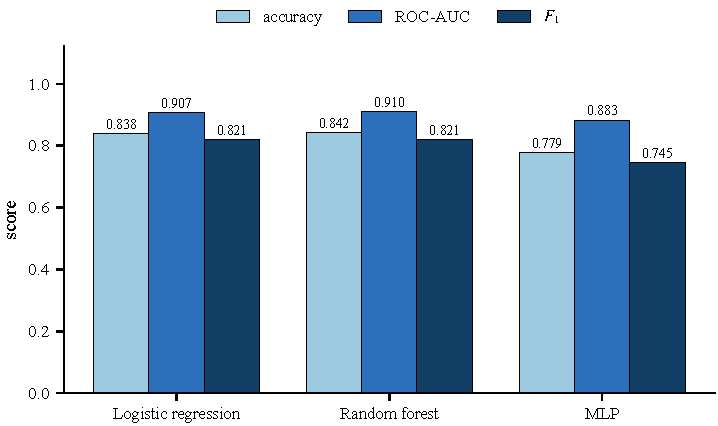
\includegraphics[width=0.62\linewidth]{fig4_internal_cleveland.pdf}
\caption{Internal Cleveland performance under stratified five-fold cross-validation with
all thirteen predictors. The two classical learners are separated by less than one
standard error of the AUC at this sample size; the neural network is not competitive.}
\label{fig:internal}
\end{figure}

Taken alone, \cref{tab:internal} would support a confident claim: an
$\mathrm{AUC}\approx0.91$ classifier for coronary artery disease. The remainder of the
paper is an argument that this claim is not yet a statement about anything outside
Cleveland.

\subsection{The transfer matrix}
\cref{fig:matrix} shows the full $4\times4$ directed matrix per model, and
\cref{tab:pairs} lists the twelve off-diagonal scores. Three structural facts stand out.

\begin{figure}[t]
\centering
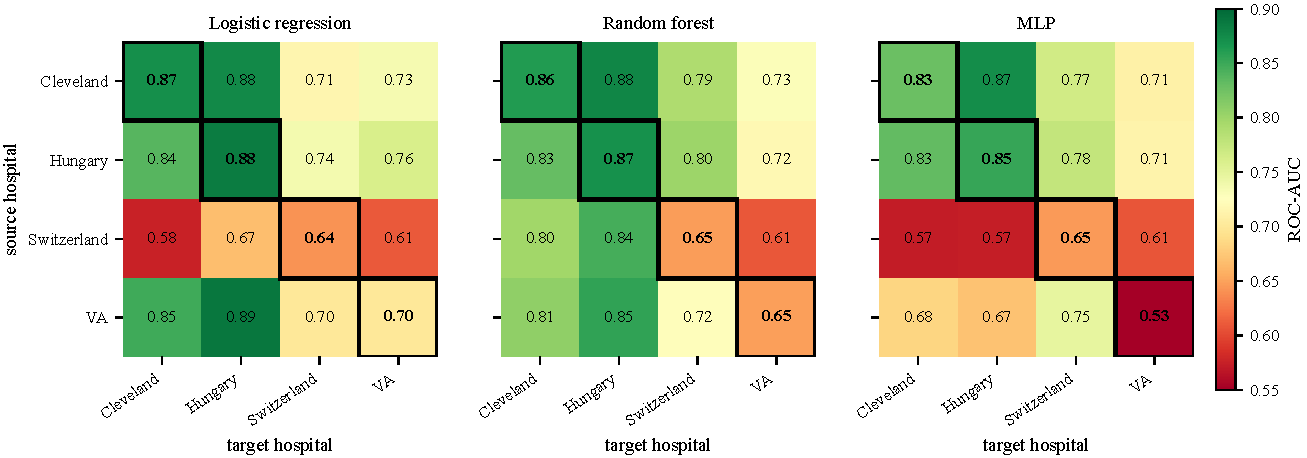
\includegraphics[width=\linewidth]{fig1_transfer_matrix.pdf}
\caption{Directed transfer matrices of ROC-AUC on the nine portable variables
($\mathcal{F}_{9}$). Rows index the source hospital used for fitting, columns the target
hospital used for scoring. Boxed diagonal cells are within-site five-fold
cross-validation with preprocessing refitted per fold; all other cells are strict
source-only fits scored on an untouched target. The dominant structure is horizontal
(source-driven), not vertical.}
\label{fig:matrix}
\end{figure}

\begin{table}[t]
\centering
\caption{All twelve directed source$\rightarrow$target transfers on $\mathcal{F}_{9}$.
Best model per row in bold.}
\label{tab:pairs}
\begin{tabular}{llrrr}
\toprule
Source & Target & Logistic & Random forest & MLP\\
\midrule
Cleveland   & Hungary     & 0.875 & \textbf{0.878} & 0.872\\
Cleveland   & Switzerland & 0.714 & \textbf{0.789} & 0.765\\
Cleveland   & VA          & \textbf{0.734} & 0.728 & 0.709\\
Hungary     & Cleveland   & \textbf{0.836} & 0.830 & 0.832\\
Hungary     & Switzerland & 0.736 & \textbf{0.799} & 0.775\\
Hungary     & VA          & \textbf{0.760} & 0.718 & 0.713\\
Switzerland & Cleveland   & 0.576 & \textbf{0.797} & 0.571\\
Switzerland & Hungary     & 0.667 & \textbf{0.844} & 0.572\\
Switzerland & VA          & \textbf{0.609} & 0.608 & 0.606\\
VA          & Cleveland   & \textbf{0.848} & 0.806 & 0.683\\
VA          & Hungary     & \textbf{0.888} & 0.854 & 0.670\\
VA          & Switzerland & 0.700 & 0.723 & \textbf{0.746}\\
\midrule
\multicolumn{2}{l}{Macro-average external} & 0.745 & \textbf{0.781} & 0.709\\
\bottomrule
\end{tabular}
\end{table}

\paragraph{Transfer is not uniformly downward}
Of the twelve directed pairs, several \emph{exceed} the corresponding internal score.
Cleveland$\rightarrow$Hungary reaches $0.875$--$0.878$, above Cleveland's own
within-site value of $0.861$--$0.870$ on the same nine features. Hungary is an easier
target: its prevalence is the lowest of the four ($0.361$) and its recorded variables are
comparatively clean. A pooled ``external AUC'' that averages Hungary together with
Switzerland conceals a factor-of-two difference in difficulty.

\paragraph{The source cohort dominates}
Reading \cref{fig:matrix} by rows rather than columns is more informative.
Switzerland as a \emph{source} is catastrophic for the two linear-ish learners: with
$93.5\%$ of Swiss patients diseased, the fitted logistic model sees almost no negative
examples and transfers at $\mathrm{AUC}=0.576$ and $0.667$ to Cleveland and Hungary---
barely above chance. The random forest, whose bootstrap resampling and balanced class
weights make it far less sensitive to an extreme prevalence, recovers $0.797$ and
$0.844$ from the same degenerate source. Conversely, Switzerland as a \emph{target} is
uniformly hard for all models ($0.700$--$0.799$), because its own outcome distribution
leaves only eight negative patients to rank against.

\paragraph{Model ranking is not stable across pairs}
Logistic regression wins five of twelve pairs, the random forest six, the MLP one. No
model dominates. A practitioner selecting a model from a single held-out target would
reach a different conclusion depending on which target they happened to hold out---which
is precisely the failure mode that motivates reporting the whole matrix.

\begin{figure}[t]
\centering
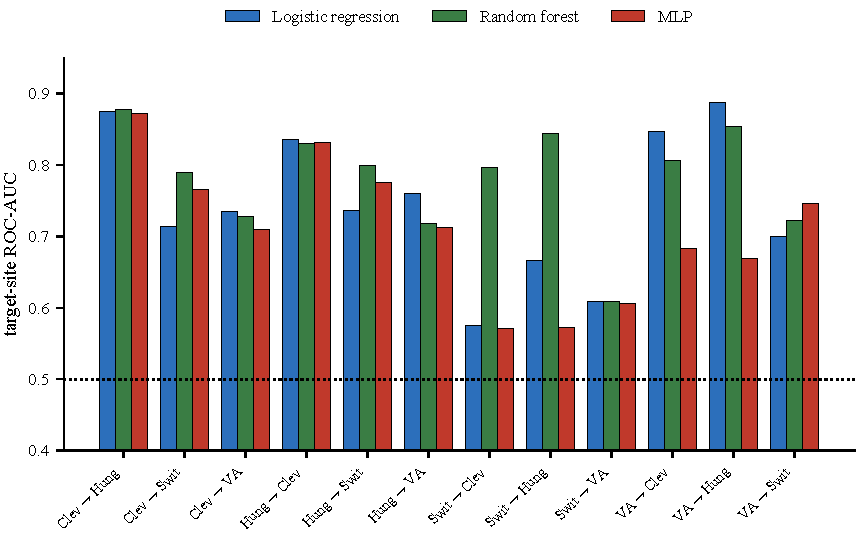
\includegraphics[width=0.86\linewidth]{fig3_directed_transfers.pdf}
\caption{The twelve directed transfers, grouped by source$\rightarrow$target pair. The
spread \emph{within} a pair (model choice) is generally smaller than the spread
\emph{across} pairs (cohort choice), except where the source cohort is degenerate
(Switzerland), in which case model choice becomes decisive.}
\label{fig:directed}
\end{figure}

\subsection{The generalization gap is not a robustness score}
\cref{tab:gap} and \cref{fig:gap} report \cref{eq:macro,eq:gap}. The random forest has
$\Delta=-0.025$: its macro-average external AUC \emph{exceeds} its macro-average
internal AUC. Read naively, this says that the random forest performs better on
hospitals it has never seen than on the hospital it was trained on, which is not a
coherent claim about robustness. The correct reading is that the two averages are taken
over different populations: the internal average is dragged down by Switzerland's
near-degenerate within-site cross-validation ($0.647$) and VA's ($0.648$), whereas the
external average includes many transfers \emph{into} the two well-behaved cohorts.

\begin{table}[t]
\centering
\caption{Macro-averaged internal and external discrimination on $\mathcal{F}_{9}$, and
the signed gap of \cref{eq:gap}. A negative gap does not indicate improvement under
shift; see \cref{sec:discussion}.}
\label{tab:gap}
\begin{tabular}{lrrr}
\toprule
Model & $\overline{A}_{\text{int}}$ & $\overline{A}_{\text{ext}}$ & $\Delta$\\
\midrule
Logistic regression & 0.774 & 0.745 & $+0.028$\\
Random forest       & 0.756 & \textbf{0.781} & $-0.025$\\
MLP                 & 0.713 & 0.709 & $+0.003$\\
\bottomrule
\end{tabular}
\end{table}

\begin{figure}[t]
\centering
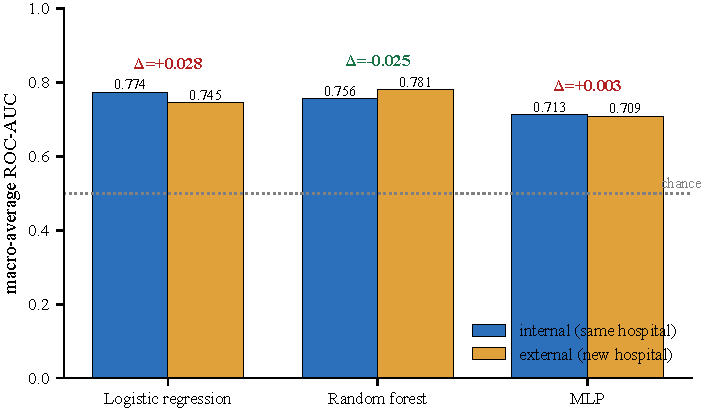
\includegraphics[width=0.66\linewidth]{fig2_generalization_gap.pdf}
\caption{Macro-averaged internal versus external discrimination. The MLP has the
smallest magnitude gap and the worst absolute performance; the random forest has a
negative gap and the best absolute external performance. Ranking models by $|\Delta|$
would select the weakest model.}
\label{fig:gap}
\end{figure}

The MLP illustrates the complementary trap. Its gap is the smallest in magnitude
($+0.003$), which under a $|\Delta|$-minimising selection rule would make it the ``most
robust'' model. But its absolute external AUC is the lowest of the three ($0.709$). A
model that is uniformly mediocre everywhere has a small gap by construction. Gap
minimisation and utility maximisation are different objectives, and only the latter is
clinically meaningful.

\section{Discussion}
\label{sec:discussion}

\subsection{What the experiment supports}
\begin{enumerate}
\item Internal discrimination on Cleveland with all thirteen variables is strong
      ($\mathrm{AUC}=0.910$).
\item Transport across these four cohorts is heterogeneous rather than uniformly
      degrading; the directed matrix is strongly asymmetric.
\item Under $\mathcal{F}_9$ the random forest achieves the highest macro-average
      external AUC in this run, and is markedly more tolerant of a degenerate source
      cohort than the linear model.
\item Source-cohort quality---size, prevalence balance, and site-specific
      missingness---explains more variance in transfer performance than model family
      does.
\end{enumerate}

\subsection{What it does not support}
The study reports no confidence intervals, no calibration
curves~\cite{vanCalster2019}, no threshold-specific sensitivity and specificity, no
subgroup audit, and no decision-curve analysis~\cite{vickers2006}. Four historical
cohorts recorded in the late 1980s do not establish contemporary clinical
generalization, and the TRIPOD reporting criteria for a deployable model are not
met~\cite{collins2015tripod}. Macro-averaging weights every directed pair equally,
which ignores that target cohorts differ in size by a factor of $2.5$ and that pairs
sharing a source are statistically dependent. With twelve directed transfers derived
from four sites, the effective number of independent external observations is four,
not twelve.

\subsection{Implications for reporting}
Three recommendations follow directly from \cref{fig:matrix}.

First, report the matrix. A single external AUC is a projection of a
$|\mathcal{S}|\times|\mathcal{S}|$ object onto one scalar, and the projection destroys
exactly the asymmetry that a deploying institution needs to see.

Second, report absolute target-site performance alongside any gap statistic. The
quantity a hospital cares about is $\mathrm{AUC}_{s\rightarrow t}$ for its own $t$, not
$\Delta$.

Third, audit the recording process before choosing a shared feature set. The Swiss
cholesterol column is a visible instance of a general hazard: a variable that is present
in the schema but absent in the data will be silently repaired by any pooled imputation
step, converting a missing-data problem into an invisible leakage problem.

\subsection{Threats to validity}
The diagonal and off-diagonal entries of \cref{fig:matrix} are estimated by different
procedures (within-site cross-validation versus a single source-only fit), so they carry
different variance. The MLP is sensitive to library version and hardware because early
stopping interacts with thread scheduling; qualitative conclusions should be drawn from
the matrix structure and not from a third decimal place. Finally, the binarisation of
\cref{eq:target} discards severity information that a graded outcome would retain.

\section{Conclusion}
External validity is a matrix of source--target behaviours, not a badge earned from one
held-out split. On the four UCI heart-disease cohorts, a model with
$\mathrm{AUC}=0.910$ under internal validation transports at anywhere between $0.571$
and $0.888$ depending on which pair of hospitals is considered, and the scalar
generalization gap is capable of ranking the weakest model first. We recommend that
multi-site clinical machine-learning studies report the full directed transfer matrix,
report absolute target performance, and treat the source cohort's recording quality as a
first-class experimental variable.

\section*{Data and Code Availability}
The cohorts are the four public UCI Heart Disease files named
\texttt{processed.\textit{site}.data}, where \textit{site} ranges over
\texttt{cleveland}, \texttt{hungarian}, \texttt{switzerland}, and
\texttt{va}. The analysis notebook,
the exported pairwise score table, and the figure-generation script accompanying this
manuscript reproduce every number reported here.

\section*{Ethical Statement}
This work uses a de-identified public benchmark. It is a methodological study of
external validation and is explicitly not a diagnostic device. No clinical decision
should be derived from any model reported here.

\bibliographystyle{ACM-Reference-Format}
\bibliography{refs}

\section*{Authors' background}

\noindent\begin{minipage}{\linewidth}
\begin{tabular}{@{}p{0.24\linewidth}p{0.18\linewidth}p{0.22\linewidth}p{0.22\linewidth}@{}}
\toprule
Your Name & Title$^{*}$ & Research Field & Personal website \\
\midrule
Anoushka Aisola  & & & \\
Vihaan Bhoopathy & & & \\
Rayan Hossain    & & & \\
Spoorthi Idumudi & & & \\
Nethra Kollipara & & & \\
Rania Malik      & & & \\
Nishant Nayagam  & & & \\
Yukti Srinivas   & & & \\
Srikanth Samy    & & & \\
Ishaan Gupta     & & & \\
\bottomrule
\end{tabular}

\vskip 6pt
{\footnotesize $^{*}$This form helps us to understand your paper better,
the form itself will not be published.\\
$^{*}$Title can be chosen from: master student, Phd candidate, assistant professor,
lecture, senior lecture, associate professor, full professor}
\end{minipage}

\end{document}
